\documentclass[11pt,a4paper]{article}
\usepackage[utf8]{inputenc}
\usepackage[margin=1in]{geometry}
\usepackage{graphicx}
\usepackage{hyperref}
\usepackage{xcolor}

\begin{document}
\noindent\textbf{\Large Tech Nation Visa - Exceptional Promise}\\
\noindent\textbf{Criteria:} Optional Criteria 3 (Product \& Engineering Impact)\\
\noindent\textbf{Applicant:} Odeyemi Olusegun Israel\\
\rule{\textwidth}{0.4pt}

\vspace{0.5cm}
\begin{center}
    \textbf{\huge Evidence 7: The AMTTP ``War Room'' Compliance Dashboard}
\end{center}
\vspace{0.5cm}

\section*{1. Enterprise-Ready Product Interface}
A core differentiator of the AMTTP platform is its bespoke compliance dashboard built with \textbf{Next.js 14 (App Router), TypeScript, and Tailwind CSS}. Designed for R3--R6 enterprise users (Compliance Officers, Risk Analysts, and Super Administrators), the ``War Room'' provides real-time surveillance over every transaction flowing through the decentralised compliance engine.

This is not a prototype or wireframe. It is a fully functional, data-driven administrative interface consuming live API responses from the Python microservice layer, rendering interactive charts, alert feeds, and risk scoring panels.

\vspace{0.3cm}
\noindent\textbf{War Room Tech Stack:}
\begin{itemize}
    \item \textbf{Framework:} Next.js 14 (App Router) + TypeScript + Tailwind CSS
    \item \textbf{Data Fetching:} TanStack React Query consuming 10+ Python FastAPI microservice endpoints
    \item \textbf{Charting:} Interactive risk score heatmaps, transaction volume timeseries, alert severity panels
    \item \textbf{Theme:} Dark mode (\texttt{bg-gray-950}) for extended surveillance sessions
    \item \textbf{Routing:} Server components by default; \texttt{'use client'} directive only for interactive panels
\end{itemize}
\vspace{0.3cm}
\begin{center}
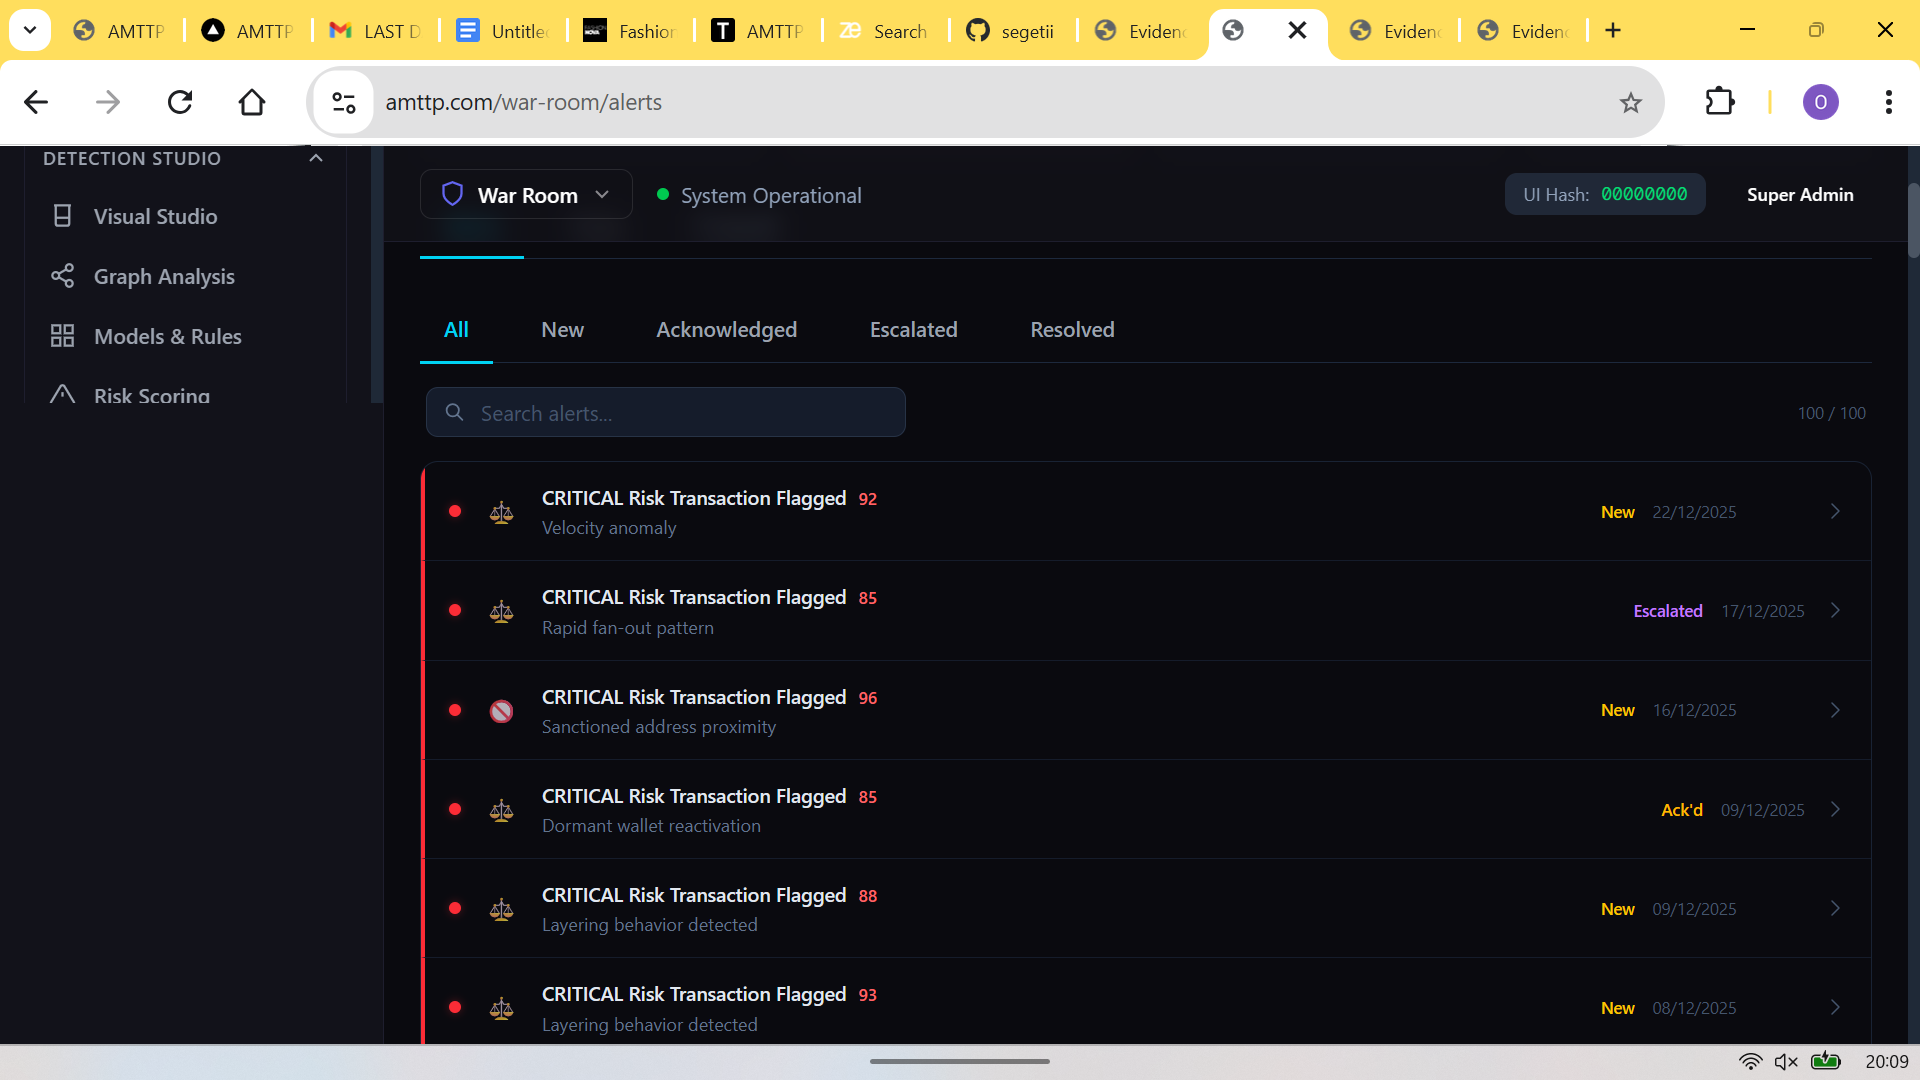
\includegraphics[width=0.95\textwidth]{images/warroom_alerts.png}
\end{center}
\vspace{0.1cm}
\textit{Figure 1: Live AMTTP War Room at \texttt{amttp.com/war-room/alerts} --- 100 CRITICAL risk transaction alerts with severity scores, status tracking (New / Escalated / Acknowledged), and pattern classification (velocity anomaly, fan-out, sanctioned address proximity, layering behavior).}

\section*{2. Role-Based Access Control (RBAC)}
The dashboard enforces a six-tier Role-Based Access Control system (R1--R6), shared via a unified JSON configuration between the Flutter consumer app and the Next.js admin panel. This ensures that end users never see compliance-sensitive data, while senior administrators have full forensic capability.

\vspace{0.3cm}
\noindent\textbf{RBAC Configuration} (from \texttt{frontend/shared/rbac\_config.json}):

\vspace{0.2cm}
\begin{center}
\begin{tabular}{|c|l|l|l|}
\hline
\textbf{Role} & \textbf{Label} & \textbf{Mode} & \textbf{Key Capabilities} \\
\hline
R1 & End User & Focus (Flutter) & Initiate own transactions only \\
R2 & PEP End User & Focus (Flutter) & Enhanced monitoring, same UI \\
R3 & Compliance Officer & War Room (Next.js) & View all transactions, reports \\
R4 & Risk Analyst & War Room (Next.js) & Detection studio, policies \\
R5 & Admin & War Room (Next.js) & Manage users, enforcement \\
R6 & Super Admin & War Room (Next.js) & Emergency override, full access \\
\hline
\end{tabular}
\end{center}
\vspace{0.2cm}

\noindent\fbox{\begin{minipage}{0.95\textwidth}
\small
\texttt{// rbac\_config.json (shared between Flutter \& Next.js)}\\
\texttt{"R1\_END\_USER": \{ "mode": "FOCUS", "canViewOthersTx": false \}}\\
\texttt{"R4\_RISK\_ANALYST": \{ "mode": "WAR\_ROOM",}\\
\texttt{~~"canAccessDetectionStudio": true, "canEditPolicies": true \}}\\
\texttt{"R6\_SUPER\_ADMIN": \{ "mode": "WAR\_ROOM",}\\
\texttt{~~"canEmergencyOverride": true, "canManageUsers": true \}}
\end{minipage}}
\vspace{0.2cm}

\noindent\textit{Figure 2: Six-tier RBAC system enforced via a single shared JSON configuration consumed by both the Flutter consumer app (R1--R2 Focus Mode) and the Next.js compliance dashboard (R3--R6 War Room Mode).}

\vspace{0.3cm}
\begin{center}
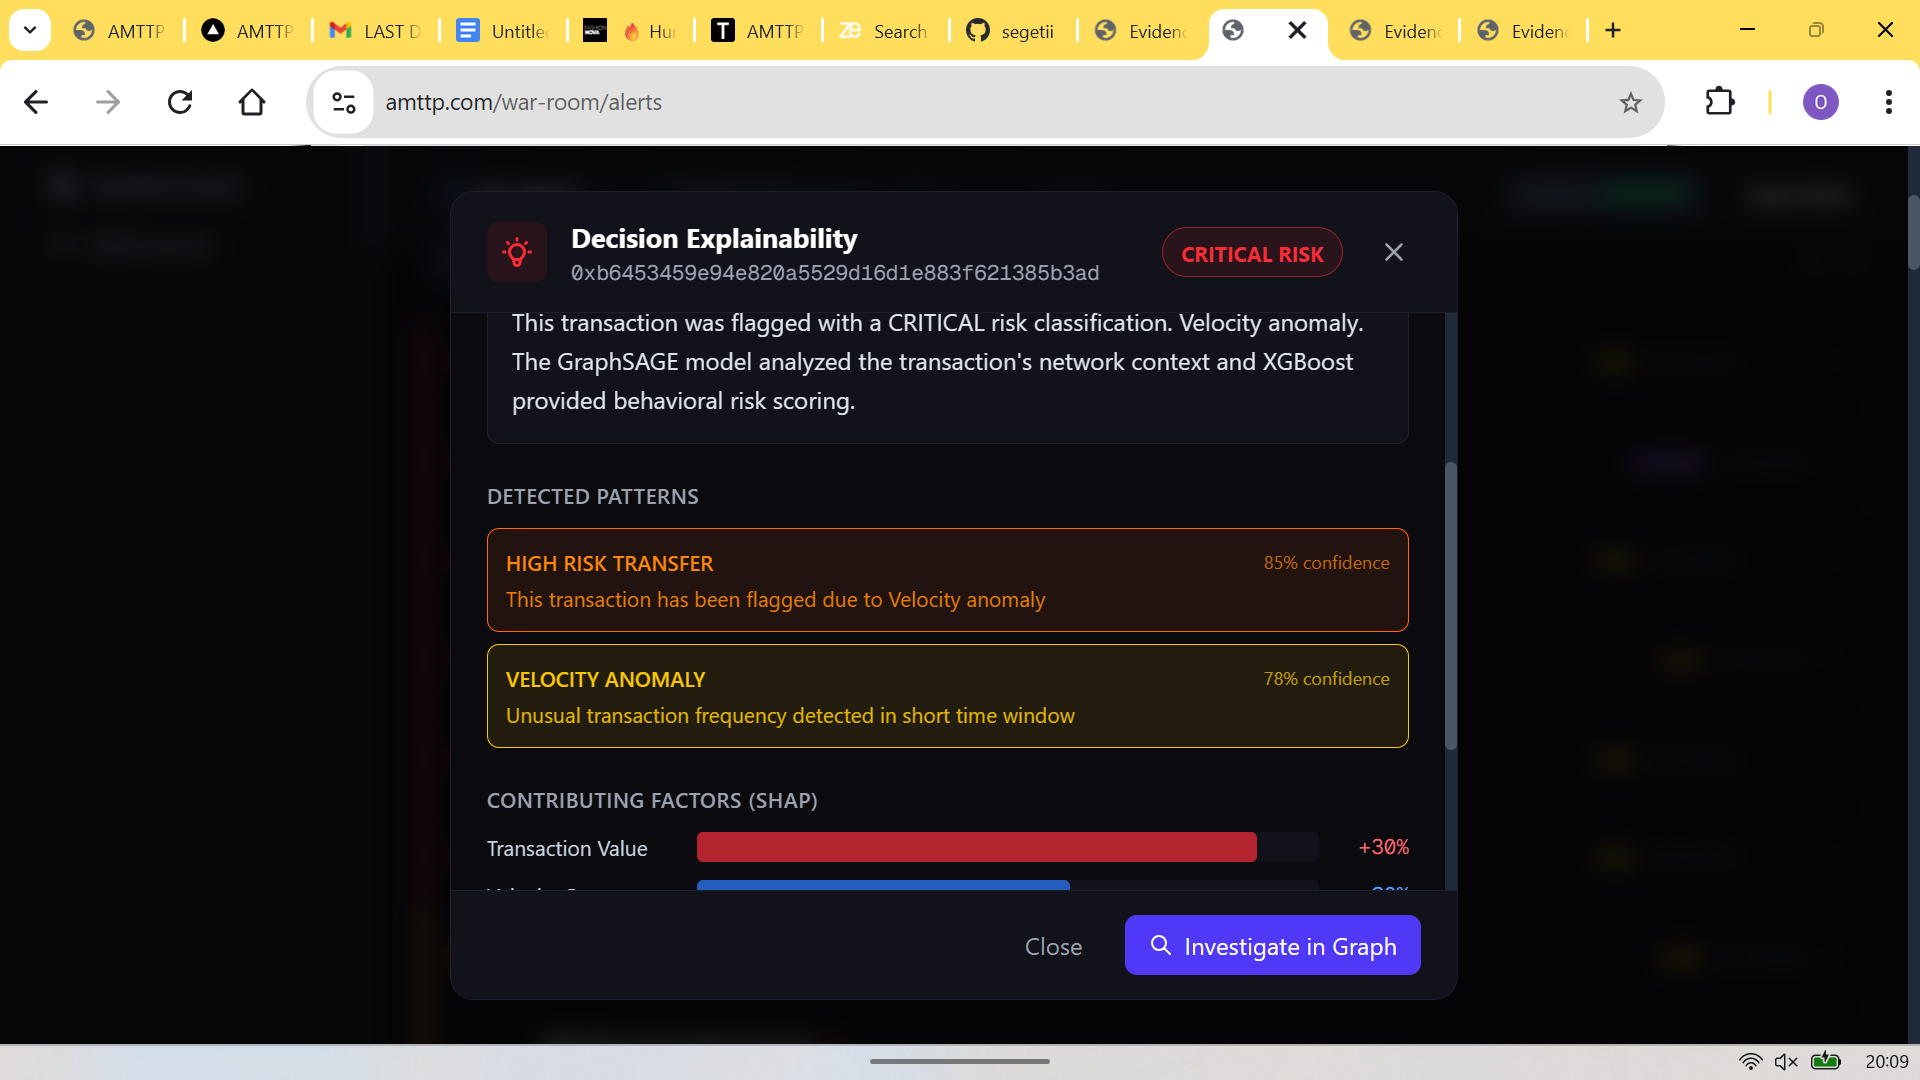
\includegraphics[width=0.85\textwidth]{images/warroom_explainability.png}
\end{center}
\vspace{0.1cm}
\textit{Figure 3: Decision Explainability panel --- SHAP-based contributing factors for a CRITICAL risk alert. Shows detected patterns (High Risk Transfer 85\%, Velocity Anomaly 78\%) with an ``Investigate in Graph'' action linking to the graph analysis engine.}

\section*{3. Technical Significance}
Building a production-quality compliance dashboard from scratch --- rather than using off-the-shelf tools like Retool or Grafana --- demonstrates deep frontend engineering capability and a commitment to owning the full product stack. Every chart, table, and alert component was hand-coded by the applicant, as evidenced by the GitHub commit history (see Evidence 5).

\end{document}